\section{Техническое задание}
\subsection{Основание для разработки}

Полное наименование системы: <<Веб-приложение \textquotedbl Социомаркет для владельцев домашних животных \textquotedbl\ >>.
Основанием для разработки программы является приказ ректора ЮЗГУ от <<24>> ноября 2023 г. №5166-с <<Об утверждении тем выпускных квалификационных работ>>.

\subsection{Цель и назначение разработки}

Веб-приложение <<Социомаркет для владельцев домашних животных>> создается с целью объединения пользователей двух групп: владельцев домашних животных и лиц, предоставляющих услуги для домашних животных. Такими лицами могут являться владельцы интернет-магазинов, предприниматели или такие же пользователи.

Задачами данной разработки являются:
\begin{itemize}
\item разработка клиентской части web-сайта;
\item создание каталогов с категориями карточек на сайте;
\item реализация формы создания и управления карточкой услуги;
\item создание удобного поиска по каталогам карточкам;
\item реализация взаимодействия между пользователями сайта;
\item разработка и развертывание инфраструктуры web-сайта и его базы данных на удаленном сервере;
\item разработка серверной части web-сайта;
\item разработка REST API для взаимодействия клиентской и серверной частей;
\item разработка базы данных.
\end{itemize}

Задачей разработки серверной части также является следования принципам, описанным в работе Марка Прайса <<C\# 9 и .NET 5. Разработка и оптимизация>> \cite{mark_price}.

\subsection{Требования пользователя к интерфейсу web-сайта}

Сайт должен включать в себя:
\begin{itemize}
    \item авторизацию;
    \item навигацию по разделам;
    \item разделение доступа к функционалу сайта для пользователя и лица предоставляющего услуги;
    \item поиск по пользователям и их товарам или услугам.
\end{itemize}


\subsection{Требования к программной системе веб-приложения <<Социомаркет>>}
\subsubsection{Требования к данным программной системы}
Система должна уметь эффективно обрабатывать данные пользователей, включая личную информацию, данные о питомцах, информацию о продуктах (товары и услуги). Необходимо обеспечить конфиденциальность и безопасность этих данных.
На рисунке  \ref{bd:image} представлена концептуальная модель данных программной системы в виде UML-диаграммы сущность-связь.

\begin{figure}[ht]
\centering
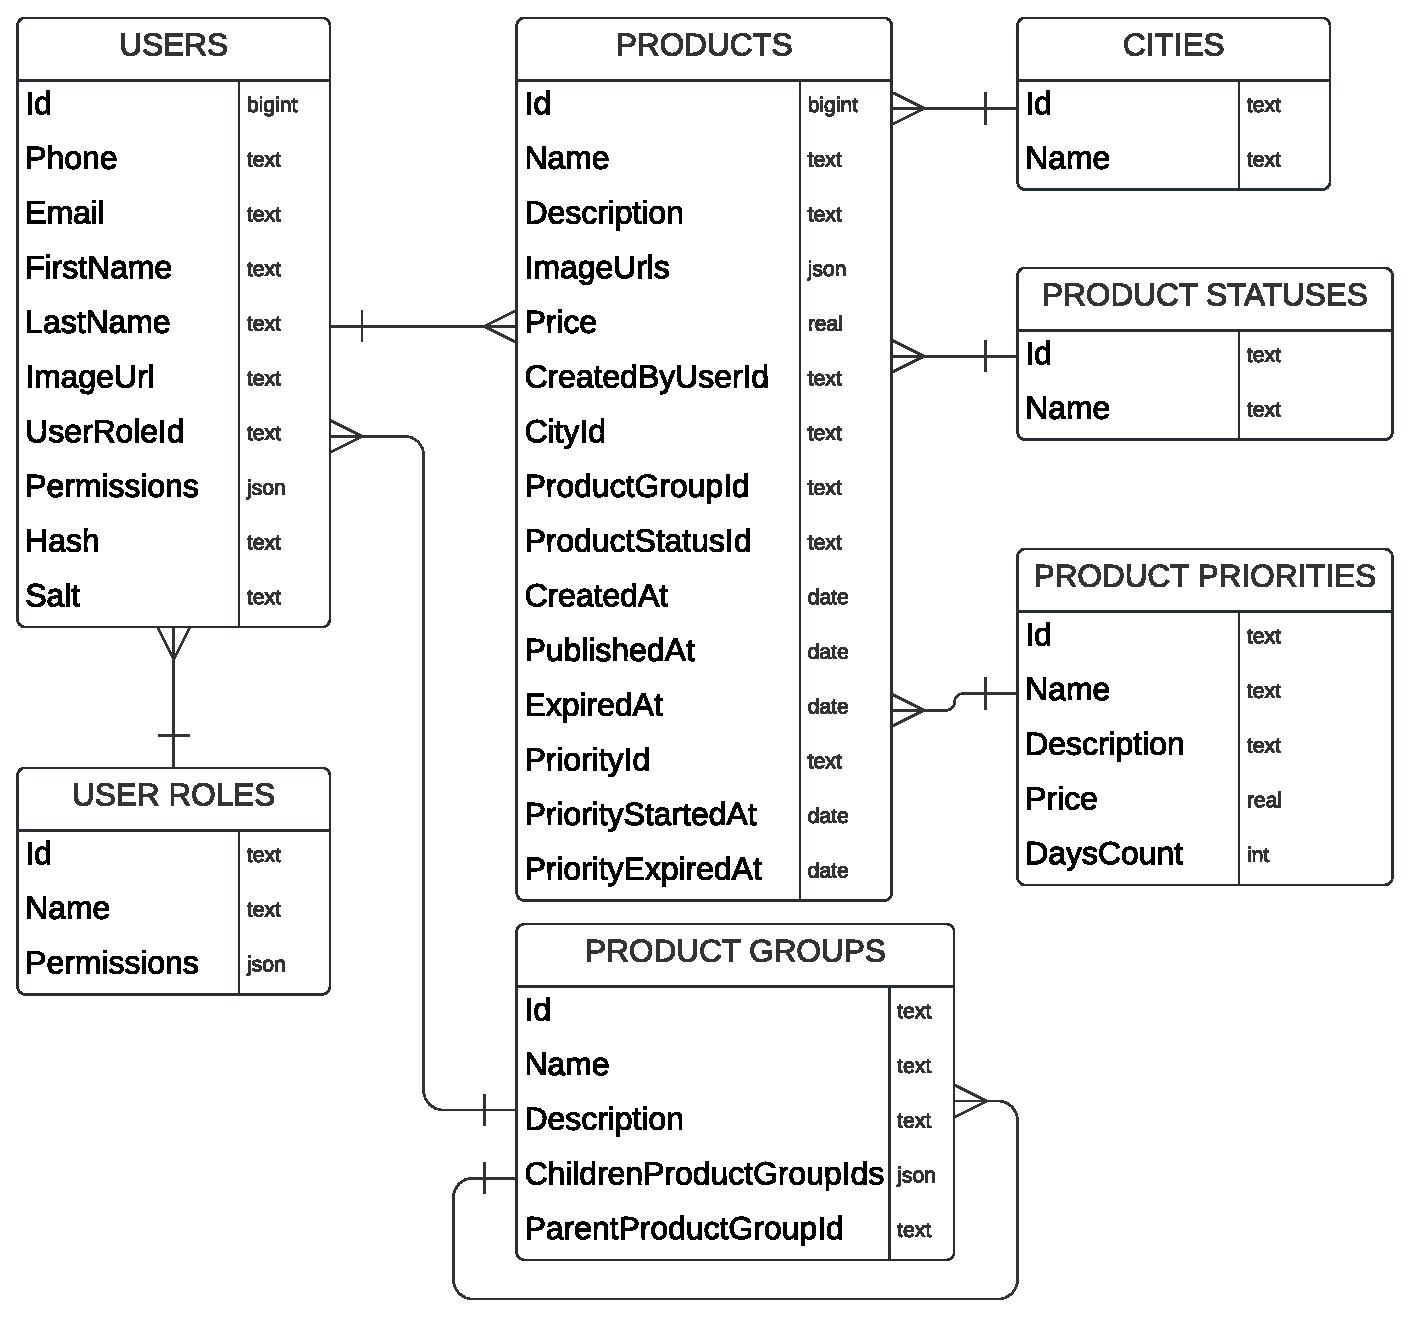
\includegraphics[width=1\linewidth]{bd}
\caption{Концептуальная модель данных}
\label{bd:image}
\end{figure}

В приведенной на рисунке \ref{bd:image} диаграмме сущность-связь представлены сущности и атрибуты, которые будут использоваться в программной системе.

Данные программной системы должны быть организованы таким образом, чтобы не разделять на 2 отдельные группы пользователей и лиц, предоставляющих услуги. Отличие между пользователями должно быть записано в атрибуте <<UserRole>> сущности <<User>>. Таким образом, в программной системе будет только одна сущность <<User>>, которая будет иметь атрибут <<UserRole>> со значениями <<SITTER>> и <<OWNER>>.
При проектировании модели данных также необходимо учесть то, что сущность <<Product>> представляет собой продукт, который может быть как товаром, так и услугой. Для этого не требуется никаких дополнительных атрибутов, так как сущность <<Product>> становится товаром или услугой в зависисмости от названия и описания карточки продукта.

\subsubsection{Архитектура системы} 
Серверная часть веб-приложения <<Социомаркет>> разработана на .NET Core, что отражает современные подходы в разработке программного обеспечения, описанные в <<C\# 9 и .NET 5. Разработка и оптимизация>> \cite{mark_price}. Клиентская часть, реализованная на Angular, взаимодействует с сервером через REST API. База данных построена на PostgreSQL и соответствует рекомендациям и методикам, изложенным в документации PostgreSQL \cite{postgresql}.

\subsubsection{Функциональные требования к программной системе}

На основании анализа предметной области, разрабатываемая программная система <<Социомаркет для владельцев домашних животных>> должна включать в себя следующие ключевые функциональные возможности:

\begin{itemize}
\item <<Регистрация с ролью: Клиент>>;
\item <<Регистрация с ролью: Продавец>>;
\item <<Поиск по карточкам>>;
\item <<Просмотр карточек>>;
\item <<Создать карточку>> -\- Предоставление функциональности для продавцов по созданию карточек, которые будут содержать всю необходимую информацию о предлагаемых товарах или услугах;
\item <<Редактировать карточку>> -\- Возможность для продавцов изменять содержимое ранее созданных карточек, чтобы информация оставалась актуальной;
\item <<Удалить карточку>> -\- Реализация опции удаления карточек для продавцов, позволяющая убирать предложения, которые более неактуальны или доступны;
\item <<Начать общение с другим пользователем о карточке>>.
\end{itemize}

Эти требования отражают основные сценарии использования системы и направлены на создание удобного и эффективного сервиса для обоих классов пользователей: клиентов и продавцов.

На рисунке \ref{people:image} представлена диаграмма прецедентов, которая служит важным средством для систематизации функциональных требований и возможностей системы, выявляя ключевые сценарии использования. Диаграмма прецедентов изображает, как пользователи могут взаимодействовать с системой, а также помогает выявить набор основных функциональных возможностей, доступных пользователям. Каждый прецедент на диаграмме отражает отдельный путь взаимодействия в системе и представляет потенциальные действия, которые могут быть предприняты пользователями в различных ролях.

\begin{figure}[ht]
\centering
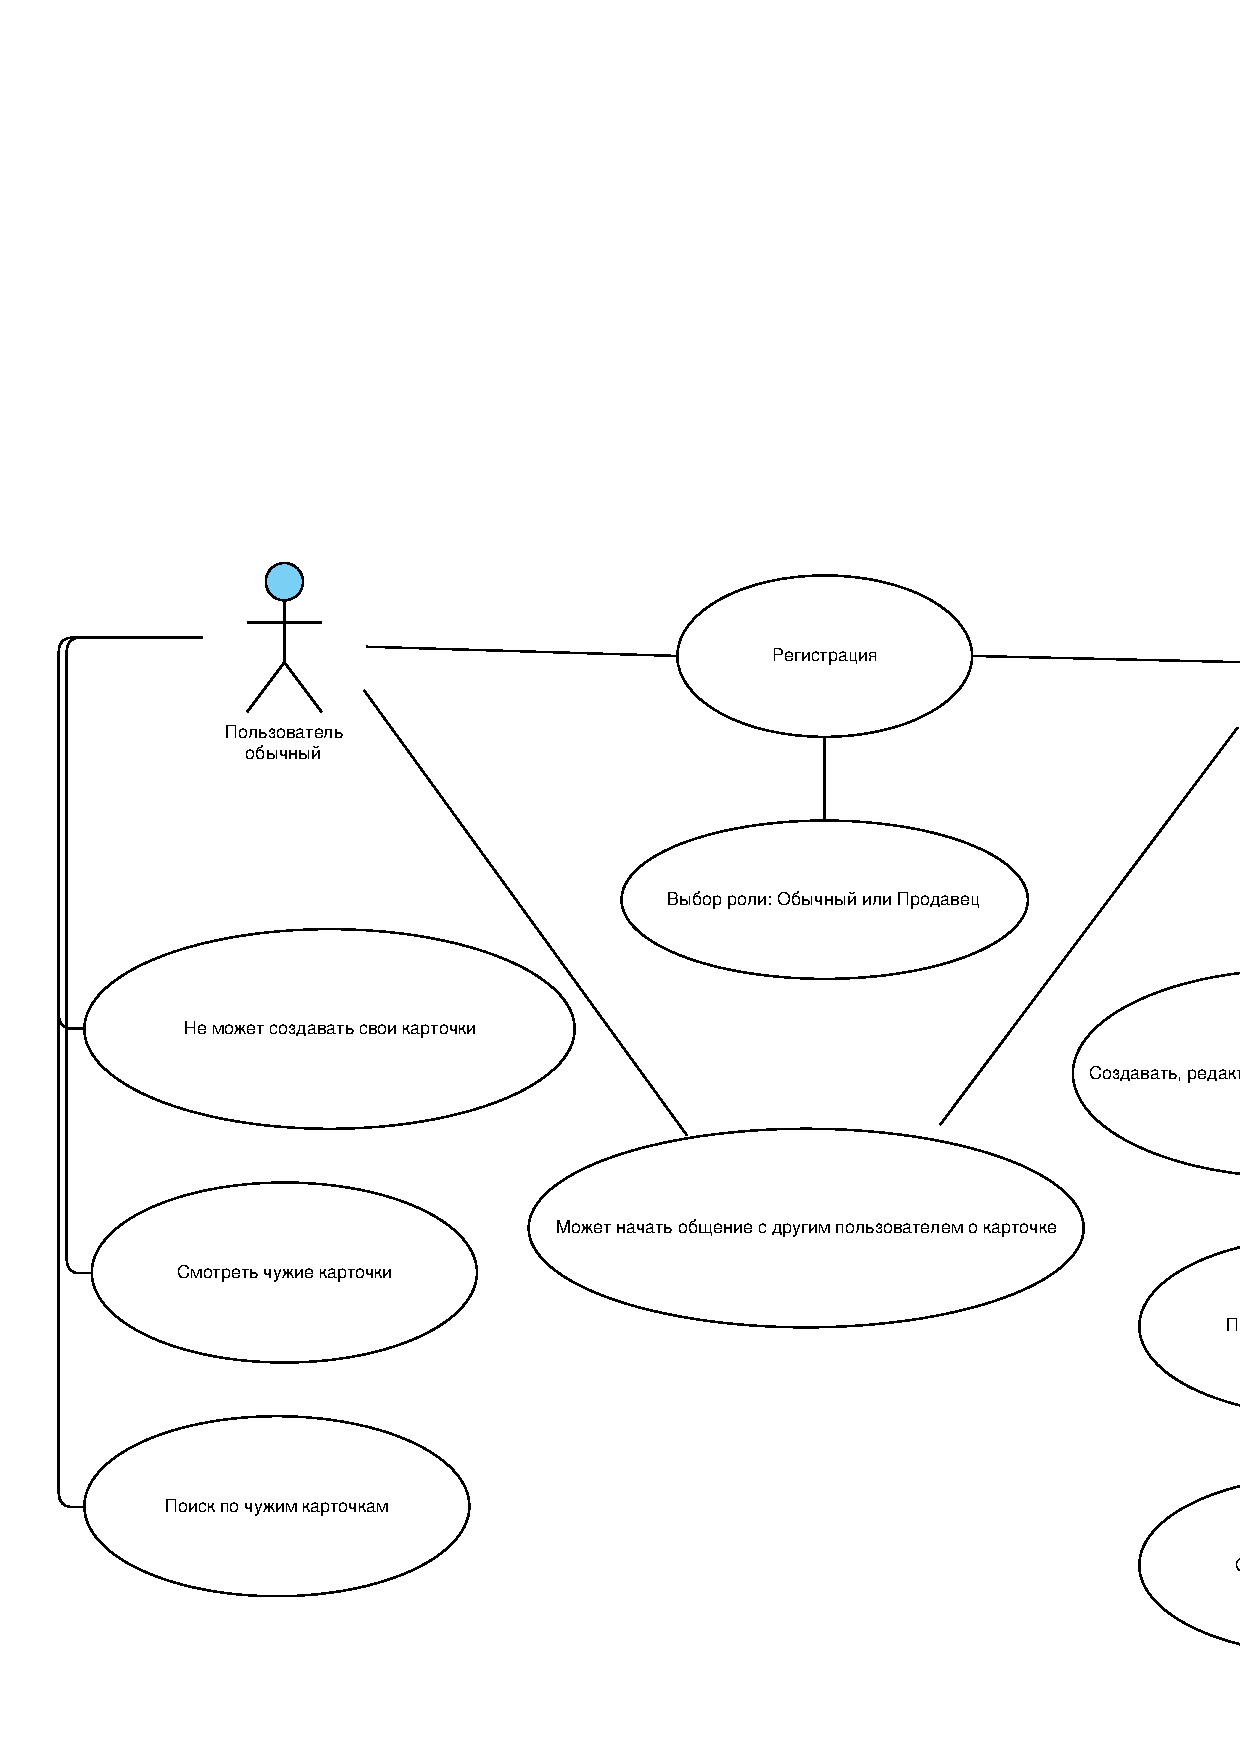
\includegraphics[width=1\linewidth]{people}
\caption{Диаграмма прецедентов}
\label{people:image}
\end{figure}

\subsubsection{Вариант использования <<Регистрация с ролью: Клиент>>}
Клиенты регистрируются в системе, предоставляя свои личные данные для создания профиля, что позволяет им пользоваться услугами платформы.

\subsubsection{Вариант использования <<Регистрация с ролью: Продавец>>}
Продавцы регистрируются в системе, указывая информацию о своих товарах и услугах, что дает им возможность размещать карточки товаров и услуг для просмотра и покупки клиентами.

\subsubsection{Вариант использования <<Поиск по карточкам>>}
Пользователи могут выполнять поиск карточек товаров и услуг с помощью ключевых слов и фильтров для нахождения наиболее подходящих предложений.

\subsubsection{Вариант использования <<Просмотр карточек>>}
Пользователи могут просматривать карточки товаров и услуг, которые содержат детальную информацию, такую как описание, цена, фотографии товаров и отзывы клиентов.

\subsubsection{Вариант использования <<Создать карточку>>}
Продавцы могут создавать карточки для своих товаров и услуг, добавляя описания, цены, фотографии и другую информацию для клиентов.

\subsubsection{Вариант использования <<Редактировать карточку>>}
Продавцы имеют возможность редактировать содержание своих карточек, обновляя информацию о товарах и услугах по мере необходимости.

\subsubsection{Вариант использования <<Удалить карточку>>}
Продавцы могут удалять свои карточки из системы, когда товар или услуга больше не доступны или не актуальны.

\subsubsection{Вариант использования <<Начать общение с другим пользователем о карточке>>}
Пользователи могут инициировать общение с другими пользователями или продавцами, чтобы узнать больше о товаре или услуге или обсудить детали сотрудничества.

\subsection{Требования пользователя к интерфейсу приложения}
Интерфейс должен быть интуитивно понятным, удобным для пользователя, с четкой навигацией и адаптивным дизайном, подходящим для различных устройств. Принципы разработки интерфейса и адаптивного дизайна основаны на спецификациях HTML и CSS, как указано в <<Спецификация CSS>> \cite{cssspecs} и <<Спецификация HTML>> \cite{htmlbook}.
При проектировании интерфейса следует отказаться от диалоговых окон для крупных элементов сайта. То есть регистрация, поиск, результат поиска - все они будут на отдельных страницах, а не внутри диалоговых окон.

\subsection{Нефункциональные требования к программной системе}

\subsubsection{Требования к надежности}
В процессе работы серверной части программной системы возможны следующие аварийные ситуации:
\begin{enumerate}
\item Потеря доступа к сети Интернет.
\item Аварийное отключение электропитания.
\item Сбой операционной системы сервера.
\end{enumerate}

Для минимизации вероятности возникновения аварийных событий серверные компоненты программной системы должны быть размещены на выделенных серверах в дата-центрах хостинг-провайдеров, прошедших сертификацию и имеющих гарантию SLA>99,8\%. Операционная системадолжна получать регулярные накопительные обновления.

\subsubsection{Требования к безопасности}
Наличие механизма проверки целостности приложения путем использования криптографических функций, основанных на подписи пакета программы. Коммуникация с сервером по защищенному протоколу.

Требования к безопасности серверной части программной системы:
\begin{enumerate}
\item Регулярные обновления компонентов безопасности операционной системы.
\item Автоматическое обновление HTTPS-сертификатов.
\item Доступ к серверу должен осуществляться без разглашения IP-адреса целевой машины в целях предотвращения возможных атак типа DDoS.
\item Запросы к серверу должны предварительно обрабатываться на одельной машине с запущенным экземпляром сервера Nginx для контроля количества запросов и логирования обращений к серверу.
\item Правилами брандмауэра операционной системы основного сервера должно быть разрешено подключение к порту сервера только с IP-адреса промежуточной машины.
\end{enumerate}

Требования к безопасности клиентской части программной системы:
\begin{enumerate}
\item Поддержка современных браузеров и операционных систем, обеспечивающая стабильную и безопасную работу на различных платформах.
\item Использование технологий адаптивной верстки приложения.
\item Реализация защиты от XSS и CSRF атак, предотвращающая нежелательное вмешательство в работу приложения.
\item Регулярное обновление компонентов системы для предотвращения уязвимостей, связанных с устаревшим программным обеспечением.
\end{enumerate}

\subsubsection{Требования к программному обеспечению}
Для реализации программной системы должны быть использованы следующие языки программирования:
С\# -\- серверная часть приложения;
Type-script -\- клиентская часть приложения;
SQL -\- язык структурированных запросов к базе данных.

Для работы клиентской части приложения требуется ОС Android 5.0 или более поздняя версия или Windows 7 или более поздняя версия с установленным браузером Google Chrome.
Для работы серверных компонентов требуется ОС Windows 7 или Macos 12.0 или Ubuntu 16.0 или более поздняя версия c установленной СУБД PostgreSQL, .NET CORE 6.0, .NET SDK 6.0.

\subsubsection{Требования к аппаратному обеспечению}
Для сервера необходим центральный процессор с количеством ядер от 6 и выше с частотой ядра от 2.4 ГГц. Объем оперативной памяти – 32 Гб. Требование к скорости интернет-соединения – 100 Мбит/c и выше.

\subsection{Требования к оформлению документации}
Требования к стадиям разработки программ и программной документации для вычислительных машин, комплексов и систем независимо от их назначения и области применения, этапам и содержанию работ устанавливаются ГОСТ 19.102–77.
Программная документация должна включать в себя:

\begin{enumerate}
\item Анализ предметной области.
\item Техническое задание.
\item Технический проект.
\item Рабочий проект.
\end{enumerate}
